\documentclass[10pt,twocolumn,twoside,openany,bg=full,layout=true,nomultitoc]{dndbook}

% Use babel or polyglossia to automatically redefine macros for terms
% Armor Class, Level, etc...
% Default output is in English; captions are located in lib/dndstring-captions.sty.
% If no captions exist for a language, English will be used.
%1. To load a language with babel:
%	\usepackage[<lang>]{babel}
%2. To load a language with polyglossia:
%	\usepackage{polyglossia}
%	\setdefaultlanguage{<lang>}
\usepackage[english]{babel}
%\usepackage[czech]{babel}
% For further options (multilanguage documents, hypenations, language environments...)
% please refer to babel/polyglossia's documentation.
\usepackage[utf8]{inputenc}
\usepackage[singlelinecheck=false]{caption}
\usepackage{lipsum}
\usepackage{listings}
\usepackage{shortvrb}
\usepackage{stfloats}
\usepackage{graphicx}
\usepackage{wrapfig}
\usepackage{multicol}
\usepackage{enumerate}
\usepackage{fancyhdr} % For customizing headers and footers
\usepackage{geometry} % For page geometry
\usepackage{background}


\captionsetup[table]{labelformat=empty,font={sf,sc,bf,},skip=0pt}

\MakeShortVerb{|}

\lstset{%
  basicstyle=\ttfamily,
  language=[LaTeX]{TeX},
  breaklines=true,
}

\begin{document}
\frontmatter
\title {Convicts' Quest\\ \large TTRPG Adventure set in Forgotten Realms}
\author {by: Tomáš Fanta}
\date {2024}



\begin{titlepage}
    \centering
    \textbf {\huge Convicts' Quest\\\large TTRPG Adventure set in Forgotten Realms\\}
    \textbf {Tomáš Fanta\\}
    \textbf {2024\\}
    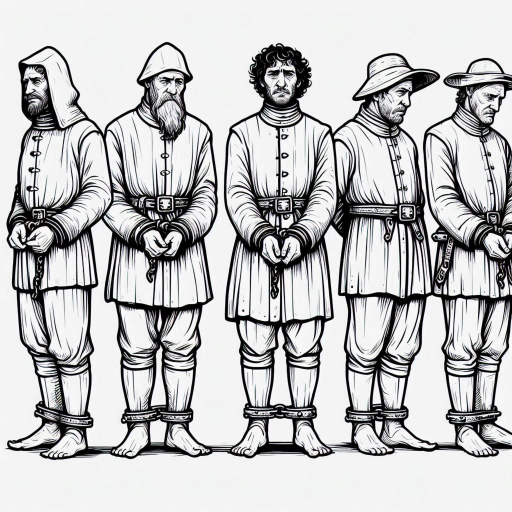
\includegraphics[width=0.5\textwidth]{img/title}\\[1cm]
    \vspace{1.5cm}
    \begin{flushleft}
      \footnotesize
      \textbf{Legal Notice:}\\
      This adventure, text documents and other materials are inspired or adapted from the following sources:\\
      - Forgotten Realms lore, 5th Edition, Wizards of the Coast.\\
      All copyrights and trademarks are owned by their respective owners.\\
      This is a fan-made adventure, that serves for non-commercial use, and I am not affiliated with Wizards of the Coast.\\
      This document is provided "as is" without warranty of any kind, either express or implied, including, but not limited to,
      the implied warranties of merchantability and fitness for a particular purpose.
      The entire risk as to the quality and performance of the document is with you.
      Should the document prove defective, you assume the cost of all necessary servicing, repair or correction.\\
      Convicts' Quest © 2024 by Tomáš Fanta is licensed under CC BY-NC-ND 4.0. To view a copy of this license, visit \texttt{https://creativecommons.org/licenses/by-nc-nd/4.0/}
    \end{flushleft}
\end{titlepage}




\tableofcontents

\mainmatter

\chapter{Introduction}\label{ch:introduction}
\DndDropCapLine{T}{his adventure is designed as introduction to DnD}
which could be enjoyed both by beginners and experienced players.
The duration may vary depending on players' pace and experience.
During my testing with two different groups, it took around 4-6 hours to finish the adventure.
The adventure is designed for 4 players with characters of 2nd level.
Please note that this is a fan-made adventure, that serves for non-commercial use, I am the author of the characters,
the story and the maps.
The rest of the content is based on the DnD 5e rules and ForgottenRealms setting, but it can be easily adapted to other
settings and TTRPG rules


\subsection*{Adventure theme}
Sandbox urban fantasy with slight vampiric influence, following the classic conflict between criminal and ruling forces,
centred particularly on cooperative storytelling with classic elements of dungeon crawling, political intrigue, light settlement building, and exploration.

\subsection*{Narative pitch}
The group of convicts who have just served their sentence of forced labour in the metropolis of Waterdeep on the shores of the Sword Coast,
attempting to cleanse their names, pay off debts, and perhaps join the elite group of adventurers who protects the city.
However, the journey will be arduous, filled with constant conflicts between the criminal underworld and city forces.
But a new player enters the scene with a growing community vying for the position of the masked lord.
The choice is yours on whom to support to achieve your goals.

\subsection*{The tone and aim of the game}
Aim for more serious cooperative storytelling, focused more on RP than on combat.
Important thing is to have fun together.

\begin{wrapfigure}{r}{0.5\textwidth}
\begin{DndComment}{General tips to make your game more enjoyable}
  \begin{enumerate}
    \item \textbf{Rule of discussion} - Everyone tries to ensure that everyone speaks for the same amount of time.
    \item \textbf{Cooperation} - DM is not playing against the players but with them.
    \item \textbf{Don't argue with DM} - If you disagree with the DM, discuss it after the game.
    \item \textbf{Do not metagame} - Do not use out-of-game knowledge in-game.
    \item \textbf{Do not cheat} - The game is about fun, not winning.
    \item \textbf{Talk in character} - It's more immersive.
    \item \textbf{Focus on the game} - take breaks if needed, set-up do-not-disturb mode.
    \item \textbf{Improvisation} - DM doesn't know everything so expect some improvisation.
  \end{enumerate}
  \end{DndComment}
\end{wrapfigure}

\newpage

\onecolumn

\chapter{Player characters}\label{ch:player-characters}
\section{Choosing a character}\label{sec:choosing-a-character}
Let players choose from these premade characters or create their own.
This is also an information everyone knows about each other.
If players choose to create their own characters, they should be from around Waterdeep and have been on forced labour with others.
They should have
After they choose, give them full backstory which includes character's secrets.


\newpage

  \section{Premade characters}\label{sec:premade-characters}
  \begin{wrapfigure}{r}{0.2\textwidth}
    \begin{center}
      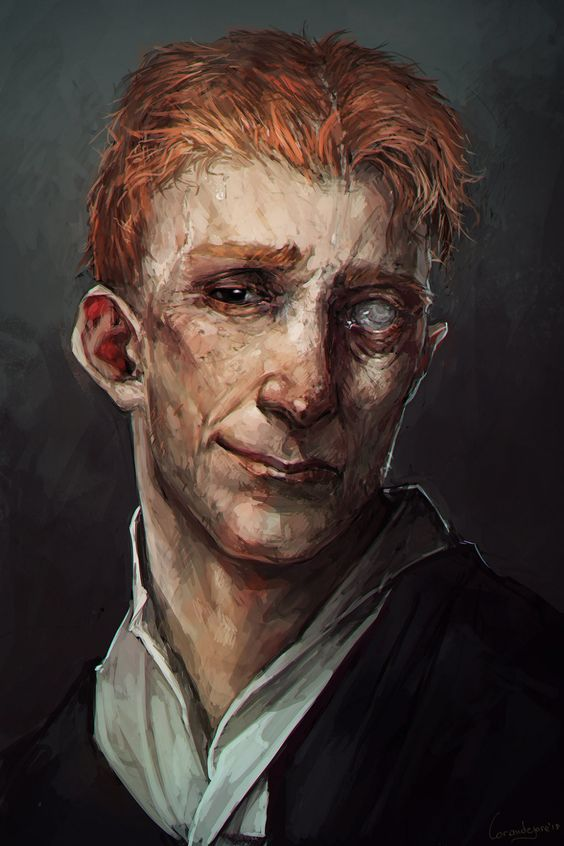
\includegraphics[width=0.2\textwidth]{img/harold}
    \end{center}
  \end{wrapfigure}
  \subsection {Harold "Scar" of Kremle}\label{subsec:harold-"scar"-of-kremle}

  \paragraph{Heavy weapons fighter}
  Despite being a lyrist, he has an unusually muscular build and strong arms, almost as if the small instrument in his
  hand might accidentally be crushed.
  Clearly familiar with both the city and the wilderness, hard work is no stranger to him.
  An ugly scar on his face gives him a rather intimidating expression more fitting for a criminal than a wandering bard,
  even though his attire and rather joyous expression might suggest otherwise.

  \begin{wrapfigure}{r}{0.2\textwidth}
    \begin{center}
      
\includegraphics[width=0.2\textwidth]{img/yasmina}
    \end{center}
  \end{wrapfigure}
  \subsection{Yasmina}\label{subsec:yasmina}

  \paragraph{Divination Wizard}
  An enthusiastic human wizard, longing for adventure, who always wears a diadem on her forehead.
  She claims to have done forced labour because she refused a powerful lecherous nobleman, and her lawyer messed it up,
  turning her from a victim into a perpetrator.
  She seems to be very clever, not ugly either, and moves as gracefully as a cat, but they've never entrusted her
  with anything heavier than a broom.
  She is knowledgeable in history and magic and has occasionally saved someone from injury thanks to her visions.


  \begin{wrapfigure}{r}{0.2\textwidth}
    \begin{center}
      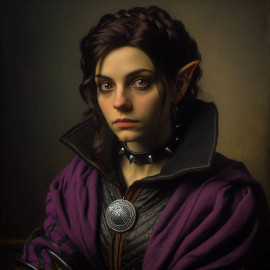
\includegraphics[width=0.2\textwidth]{img/silgrid}
    \end{center}
  \end{wrapfigure}
  \subsection{Silgrid Coalbraid}\label{subsec:silgrid-coalbraid}

  \paragraph{Dwarven rogue} A trusting, devout dwarf with a dark metal collar.
  She exudes compassion and understanding, but she might be a bit of a weirdo; I feel like she experiences other
  people's emotions too intensely.
  Unlike other dwarves, she's rather small and slender, probably wouldn't last long
  in the mines, but she moves quickly and has a good aim.
  She often discreetly prays in dark alleys when nobody's looking.
  She always wears a dark clothes, and despite all her strange quirks, she's quite easy to talk to.


  \begin{wrapfigure}{r}{0.2\textwidth}
    \begin{center}
      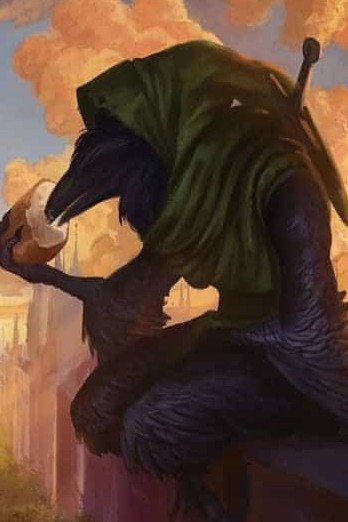
\includegraphics[width=0.2\textwidth]{img/sally}
    \end{center}
  \end{wrapfigure}
  \subsection{Sally “Jackdaw” Horst}\label{subsec:sally-jackdaw-horst}

  \paragraph{Kenku ranger, druid fighting style}
  A secretive grey-black Kenku rumoured to have once been part of the city watch.
  Unable to speak, only mimics other voices and sounds.
  Not very strong, which isn't unusual for a bird-like race.
  Appears to act with caution and not be overly swayed by emotions.
  Moves calmly and carefully observes the surroundings, alert to every rustle.
  Seems to have a grasp of nature and remains unfazed by anything in the city.
  He values morality highly and despises all criminal activities.


\pagebreak


\chapter{Character backstories}\label{ch:character-backstories}
\section{Harold "Scar" of Kremle}\label{sec:harold-"scar"-of-kremle}
\subsection{Backstory}\label{subsec:harold-backstory}
\begin{wrapfigure}{r}{0.4\textwidth}
  \begin{center}
    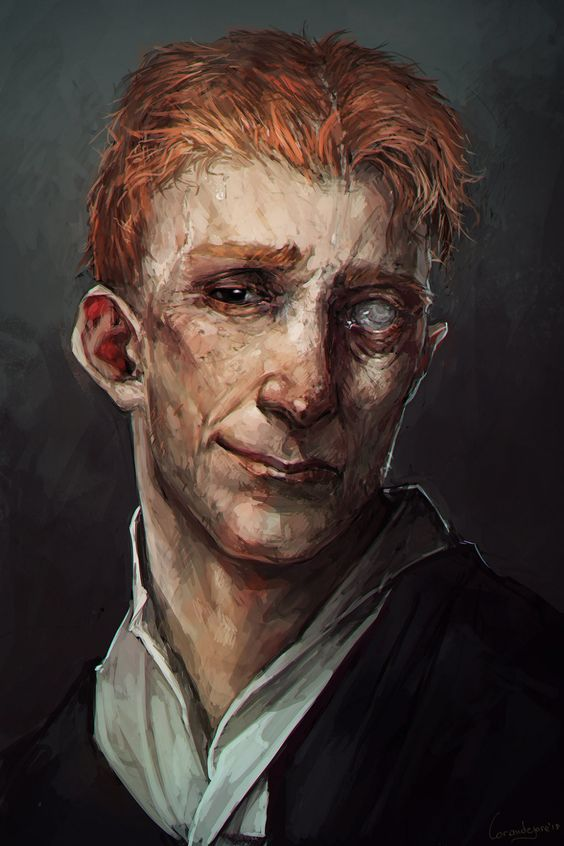
\includegraphics[width=0.4\textwidth]{img/harold}
    \vspace{1cm}
  \end{center}
\end{wrapfigure}
Harold was born in the forest village of Kremle, to a hunter's wife.
He spent most of his childhood in the woods with his father, who taught him everything about nature, survival, and hunting.
In his teens, he yearned to experience life in the city, which his father so despised.
He spent much time in the taverns of the nearby small town of Grapewade,
where he unsuccessfully tried to perform as a solo lyrist, hoping to travel the world as a wandering bard.
Due to criticism in the tavern, he often got into fights, and once he got hit by a broken bottle to the face.
Since then, they called him nothing but "Scar".
Despite not being naturally endowed with beauty or charisma, he ventured into the metropolis of Waterdeep, after a
quarrel with his Firbolg girlfriend, from whom he learned the language of giants.
In Waterdeep, he failed as a bard, and to make a living, he started doing what he knew best - hunting.
He lived in the city and hunted people or other beings, spending his free time in taverns or with esteemed music teachers.
After being tricked by his rival, a human bounty hunter named Ray Cox, into kidnapping an innocent woman and
being reported to the guards, Harold was sentenced to a year of hard labour and a ban on bounty hunting.
Now, after serving his sentence, Harold longs to rid himself of that dirty trade finally, and the only more
lucrative option to afford teachers and finally achieve fame as a musician is to become an adventurer.
\subsubsection{Secrets}
  \begin{itemize}
    \item He conceals his past as a bounty hunter
    \item He was pretending to be a musician, although he was not very good at it (even after years, he still made mistakes).
    \item He certainly lacks bardic abilities but tries to socialise as a typical bard would.
  \end{itemize}

\newpage


\section{Yasmina}\label{sec:yasmina}
\subsection{Backstory}\label{subsec:yasmina-backstory}
\begin{wrapfigure}{r}{0.4\textwidth}
  \begin{center}
    
\includegraphics[width=0.4\textwidth]{img/yasmina}
    \vspace{1cm}
  \end{center}
\end{wrapfigure}
Born as an unwanted child of a sea elf mercenary and a human sorceress who studied marine magical phenomena on the
island of Mintarn near the Sword Coast.
Shortly after birth, her father disowned her, and with her mother, she sailed
to Neverwinter, where she spent most of her childhood.\\
Her mother was ashamed of her romance with Yasmina's father, so she disguised her daughter.
To conceal her origin, she created an enchanted diadem that adjusted the shape of her ears, concealed her gills,
and changed the colour of her skin from green-blue to a human fair complexion.\\
Magic ran in her blood, and she learned everything she could from her mother and later from private tutors at the
House of Knowledge.
Because of her mother's influence, she distrusted men, especially elves, travellers, adventurers, and mercenaries.\\
Her talent for divination magic manifested during puberty, and she began to exploit it as much as she could.
In dubious ventures, she posed as a wealthy merchant, winning bets thanks to her limited knowledge of the future.
She was exposed by an older tiefling woman named Larsa, who blackmailed her into smuggling magical items and
participating in various scams.
Before Larsa was imprisoned for organizing an illegal cult worshipping demonic forces, Yasmina managed to learn
everything from her and also express unrequited love for her.
When she confessed to her mother what she had got herself into, she was thrown out of the house.\\
Using magic and deception, Yasmina managed to acquire a wagon and a donkey and set out southward.
She read fortunes for travellers and mocked, tricked and swindled arrogant adventurers, mercenaries, or soldiers,
but tried to help the poor and women.\\
In the city of Waterdeep, she completely succumbed to her hobby of disguising and deceiving people.
She got into debt, bought all the necessary luxury clothing and accessories, forged documents, and began to impersonate
a local noblewoman to acquire her estate and a comfortable life.
In the end, she took too much risk and offended an influential man (Arnold Klinger), who uncovered her disguise.
She very unpleasantly bribed the lecherous judge Methodius, and instead of whipping and imprisonment,
she had to do forced labour for a year.\\
All she had left was a magical diadem, her personal belongings, and a hefty debt (500 gold) to a loan shark named "Goldsmith."\\
She decided to take a break from illegal activities and reluctantly admitted that the only way to make big money was
to become an adventurer.
She disguised herself as an enthusiastic wizard who craved adventure.

\subsubsection{Secrets}\label{subsec:yasmina-secrets}
\begin{itemize}
\item She conceals her fraudulent past as well as her racial identity she is ashamed of.
\item She poses as an enthusiastic wizard while, in reality, she is cynical and greedy.
\item The only ones she cares about are women in distress and the poor, but she also tries to hide that,
this might be the only thing which would make her become an honest good person.
\end{itemize}

\newpage


\section{Silgrid Coalbraid}\label{sec:silgrid-coalbraid}
\subsection{Backstory}\label{subsec:silgrid-backstory}
\begin{wrapfigure}{r}{0.4\textwidth}
  \begin{center}
    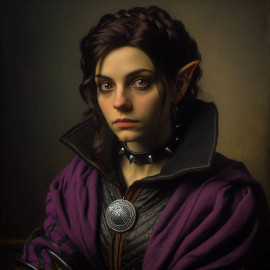
\includegraphics[width=0.4\textwidth]{img/silgrid}
    \vspace{1cm}
  \end{center}
\end{wrapfigure}

Born in the Troll Mountains in an underground settlement of gold and shield dwarves.
The settlement often faced attacks from drow and goblins, resulting in the deaths of many of her clanmates and friends,
leading her to become apathetic and suppress all grief within herself.
She limited her contact with others and immersed herself in her destructive craft - mining alchemy.\\

The population of the settlement decreased so much that the council of elders decided to destroy the village and mines
and seek refuge in the nearby trade city of Easting.\\

Feeling lonely and full of unexpressed sorrow in a foreign city on the surface, Silgrid succumbed to the preaching and
manipulations of Nemio, the leader of the local secret sect of the goddess of loss and darkness, Shar.
In the underground hideout, she trained and served as a scout and soldier for the cult.
She prayed to forget the suffering of her clanmates and the loss of her home.
The pounding on the stone gate, calling for help, the roar of Rhûn, her love, when a horde of goblins overwhelmed him.
But blessings did not come, and she believed that only through devoted service could she gain the favour of the goddess Shar.
At the command of Nemio, she slew many, including goblins and fanatics trying to suppress freedom of worship.\\

She eventually processed her emotions and adopted a new outlook on the world.
She argued that loss is a great opportunity for a new and better beginning and that without darkness there is no light.
For her overly positive views on loss and darkness and her desire to help others cope with their loss,
she was labelled a heretic and banished.\\

Furious, Nemio, the high priestess, had her whipped as a farewell gesture left her only with a modest black garment
and placed a cursed black iron collar on her.\\

She took exile as a new beginning and an opportunity to help.
However, the curse of the collar soon manifested, and she experienced the suffering of the people she encountered in her dreams.\\

In Waterdeep, she sought ways to remove the collar.
She believed that with the help of magic, it could be done.
She had no access to mage services, so she "borrowed" a magical wand from one wizard named Forts.
However, the wand did not break the collar, and in a weak moment, Silgrid went to apologize and return the wand,
intoxicated by a strong dose of liquor.
The offended mage immediately summoned the city guard, and it wasn't long before the dwarf was performing forced labour
and had a debt of 200 gold pieces for the fine.\\

After a year of suffering, she decided to try something more honourable and decided to seek work as an adventurer
to pay off her debt and perhaps meet a mage who could help her remove the collar.\\

\subsubsection{Secrets}
\begin{itemize}
  \item Former cultist
  \item A black iron collar that cannot be removed
  \begin{itemize}
    \item The character strongly empathizes with the sorrow, suffering, and depression of characters within a 5-foot radius
  \end{itemize}
\item Worships Shar
\end{itemize}

\newpage


  \section{Sally "Jackdaw" Horst}\label{sec:sally-jackdaw-horst}
  \subsection{Backstory}\label{subsec:sally-backstory}
  \begin{wrapfigure}{r}{0.4\textwidth}
    \begin{center}
      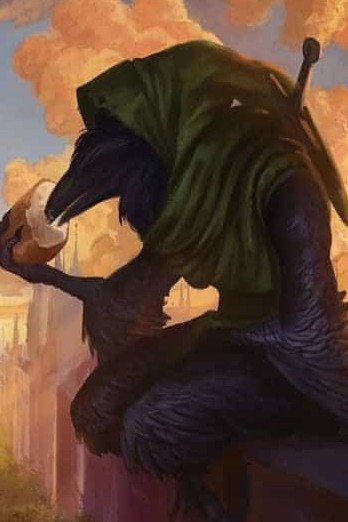
\includegraphics[width=0.4\textwidth]{img/sally}
      \vspace{1cm}
    \end{center}
  \end{wrapfigure}

He was born as a human into a family of a kind merchant dealing in glass and ceramics, located on the border between the
commercial and port districts of the city of Waterdeep.
When he was little, his parents took in an orphan who had tried to steal from their shop, so Sally suddenly had an
older brother.
Throughout their childhood, they engaged in innocent mischief and explored every corner of the city.\\

As Sally began perceiving criminal elements' influence on the city, he desired to change the situation.
He studied at the military academy and joined the city watch, eventually rising to the rank of investigator.\\

During the investigation of the disappearance of children in the impoverished district, he believes an unknown entity
cursed him.
He began to transform into an avian form until he appeared like a grey-black feathered Kenku.
With this transformation, he gained natural magical abilities and the natural skills of Kenkus, losing his ability
to speak.\\

After the transformation, he occasionally lost consciousness and woke up with bloody talons,
hearing a bird-like voice in his head.
He discovered that he hunted criminals at night, using his newfound skills.
When his nocturnal activities were discovered, he received a symbolic mild punishment—a year of forced labour and
expulsion from the city guard.\\

During his sentence, his brother Larry fell ill and could no longer manage his work as a merchant,
which Sally took over from his father.
Sally has a desire to help his brother and will financially support him if possible.\\

Becoming an adventurer was a clear choice for him—a chance for great wealth, doing good deeds, and the opportunity to
explore and master his animalistic self.\\

\subsubsection{Secrets}
\begin{itemize}
  \item The human investigator's origin
  \item Crimes committed on criminals, subconsciously during his uncontrolled transformation
  \item Voice in his head which he hears after losing control
  \item He believes he is cursed, but he knows very little about it
\end{itemize}


\newpage

\twocolumn
% example template starts bellow %

\chapter{Section}

\DndDropCapLine{T}{his example is designed to aid you in} writing beautifully typeset documents for the fifth edition of the world's greatest roleplaying game. It starts by adjusting the section formatting from the defaults in \LaTeX{} to something a bit more familiar to the reader. The chapter formatting is displayed above.

\section{Section}
Sections break up chapters into large groups of associated text.

\subsection{Subsection}
Subsections further break down the information for the reader.

\subsubsection{Subsubsection}
Subsubsections are the furthest division of text that still have a block header. Below this level, headers are displayed inline.

\paragraph{Paragraph}
The paragraph format is seldom used in the core books, but is available if you prefer it to the ``normal'' style.

\subparagraph{Subparagraph}
The subparagraph format with the paragraph indent is likely going to be more familiar to the reader.

\section{Special Sections}
The module also includes functions to aid in the proper typesetting of multi-line section headers: |\DndFeatHeader| for feats, |\DndItemHeader| magic items and traps, and |\DndSpellHeader| for spells.

\DndFeatHeader{Typesetting Savant}[Prerequisite: \LaTeX{} distribution]
You have acquired a package which aids in typesetting source material for one of your favorite games. You have advantage on Intelligence checks to typeset new content. On a failed check, you can ask questions online at the package's website.

\DndItemHeader{Foo's Quill}{Wondrous item, rare}
This quill has 3 charges. While holding it, you can use an action to expend 1 of its charges. The quill leaps from your hand and writes a contract applicable to your situation.

The quill regains 1d3 expended charges daily at dawn.

\DndSpellHeader%
  {Beautiful Typesetting}
  {4th-level illusion}
  {1 action}
  {5 feet}
  {S, M (ink and parchment, which the spell consumes)}
  {Until dispelled}
You are able to transform a written message of any length into a beautiful scroll. All creatures within range that can see the scroll must make a wisdom saving throw or be charmed by you until the spell ends.

While the creature is charmed by you, they cannot take their eyes off the scroll and cannot willingly move away from the scroll. Also, the targets can make a wisdom saving throw at the end of each of their turns. On a success, they are no longer charmed.

\section{Map Regions}
The map region functions |\DndArea| and |\DndSubArea| provide automatic numbering of areas.

\DndArea{Village of Hommlet}
This is the village of hommlet.

\DndSubArea{Inn of the Welcome Wench}
Inside the village is the inn of the Welcome Wench.

\DndSubArea{Blacksmith's Forge}
There's a blacksmith in town, too.

\DndArea{Foo's Castle}
This is foo's home, a hovel of mud and sticks.

\DndSubArea{Moat}
This ditch has a board spanning it.

\DndSubArea{Entrance}
A five-foot hole reveals the dirt floor illuminated by a hole in the roof.

\chapter{Text Boxes}

The module has three environments for setting text apart so that it is drawn to the reader's attention. |DndReadAloud| is used for text that a game master would read aloud.

\begin{DndReadAloud}
  As you approach this module you get a sense that the blood and tears of many generations went into its making. A warm feeling welcomes you as you type your first words.
\end{DndReadAloud}

\section{As an Aside}
The other two environments are the |DndComment| and the |DndSidebar|. The |DndComment| is breakable and can safely be used inline in the text.

\begin{DndComment}{This Is a Comment Box!}
  A |DndComment| is a box for minimal highlighting of text. It lacks the ornamentation of |DndSidebar|, but it can handle being broken over a column.
\end{DndComment}

The |DndSidebar| is not breakable and is best used floated toward a page corner as it is below.

\begin{DndSidebar}[float=!b]{Behold the DndSidebar!}
  The |DndSidebar| is used as a sidebar. It does not break over columns and is best used with a figure environment to float it to one corner of the page where the surrounding text can then flow around it.
\end{DndSidebar}

\section{Tables}
The |DndTable| colors the even rows and is set to the width of a line by default.

\begin{DndTable}[header=Nice Table]{XX}
    \textbf{Table head}  & \textbf{Table head} \\
    Some value  & Some value \\
    Some value  & Some value \\
    Some value  & Some value
\end{DndTable}

\chapter{Monsters and NPCs}

% Monster stat block
\begin{DndMonster}[float*=b,width=\textwidth + 8pt]{Monster Foo}
  \begin{multicols}{2}
    \DndMonsterType{Medium aberration (metasyntactic variable), neutral evil}

    % If you want to use commas in the key values, enclose the values in braces.
    \DndMonsterBasics[
        armor-class = {9 (12 with \emph{mage armor})},
        hit-points  = {\DndDice{3d8 + 3}},
        speed       = {30 ft., fly 30 ft.},
      ]

    \DndMonsterAbilityScores[
        str = 12,
        dex = 8,
        con = 13,
        int = 10,
        wis = 14,
        cha = 15,
      ]

    \DndMonsterDetails[
        %saving-throws = {Str +0, Dex +0, Con +0, Int +0, Wis +0, Cha +0},
        %skills = {Acrobatics +0, Animal Handling +0, Arcana +0, Athletics +0, Deception +0, History +0, Insight +0, Intimidation +0, Investigation +0, Medicine +0, Nature +0, Perception +0, Performance +0, Persuasion +0, Religion +0, Sleight of Hand +0, Stealth +0, Survival +0},
        %damage-vulnerabilities = {cold},
        %damage-resistances = {bludgeoning, piercing, and slashing from nonmagical attacks},
        %damage-immunities = {poison},
        %condition-immunities = {poisoned},
        senses = {darkvision 60 ft., passive Perception 10},
        languages = {Common, Goblin, Undercommon},
        challenge = 1,
      ]
    % Traits
    \DndMonsterAction{Innate Spellcasting}
    Foo's spellcasting ability is Charisma (spell save DC 12, +4 to hit with spell attacks). It can innately cast the following spells, requiring no material components:
    \begin{DndMonsterSpells}
      \DndInnateSpellLevel{misty step}
      \DndInnateSpellLevel[3]{fog cloud, rope trick}
      \DndInnateSpellLevel[1]{identify}
    \end{DndMonsterSpells}

    \DndMonsterAction{Spellcasting}
    Foo is a 2nd-level spellcaster. Its spellcasting ability is Charisma (spell save DC 12, +4 to hit with spell attacks). It has the following sorcerer spells prepared:
    \begin{DndMonsterSpells}
      \DndMonsterSpellLevel{blade ward, fire bolt, light, shocking grasp}
      \DndMonsterSpellLevel[1][3]{burning hands, mage armor, shield}
    \end{DndMonsterSpells}

    \DndMonsterSection{Actions}
    \DndMonsterAction{Multiattack}
    The foo makes two melee attacks.

    %Default values are shown commented out
    \DndMonsterAttack[
      name=Dagger,
      %distance=both, % valid options are in the set {both,melee,ranged},
      %type=weapon, %valid options are in the set {weapon,spell}
      mod=+3,
      %reach=5,
      %range=20/60,
      %targets=one target,
      dmg=\DndDice{1d4+1},
      dmg-type=piercing,
      %plus-dmg=,
      %plus-dmg-type=,
      %or-dmg=,
      %or-dmg-when=,
      %extra=,
    ]

    %\DndMonsterMelee calls \DndMonsterAttack with the melee option
    \DndMonsterMelee[
      name=Flame Tongue Longsword,
      mod=+3,
      %reach=5,
      %targets=one target,
      dmg=\DndDice{1d8+1},
      dmg-type=slashing,
      plus-dmg=\DndDice{2d6},
      plus-dmg-type=fire,
      or-dmg=\DndDice{1d10+1},
      or-dmg-when=if used with two hands,
      %extra=,
    ]

    %\DndMonsterRanged calls \DndMonsterAttack with the ranged option
    \DndMonsterRanged[
      name=Assassin's Light Crossbow,
      mod=+1,
      range=80/320,
      dmg=\DndDice{1d8},
      dmg-type=piercing,
      %plus-dmg=,
      %plus-dmg-type=,
      %or-dmg=,
      %or-dmg-when=,
      extra={, and the target must make a DC 15 Constitution saving throw, taking 24 (7d6) poison damage on a failed save, or half as much damage on a successful one}
    ]

    % Legendary Actions
    \DndMonsterSection{Legendary Actions}
    The foo can take 3 legendary actions, choosing from the options below. Only one legendary action option can be used at a time and only at the end of another creature's turn. The foo regains spent legendary actions at the start of its turn.

    \begin{DndMonsterLegendaryActions}
      \DndMonsterLegendaryAction{Move}{The foo moves up to its speed.}
      \DndMonsterLegendaryAction{Dagger Attack}{The foo makes a dagger attack.}
      \DndMonsterLegendaryAction{Create Contract (Costs 3 Actions)}{The foo presents a contract in a language it knows and waves it in the face of a creature within 10 feet. The creature must make a DC 10 Intelligence saving throw. On a failure, the creature is incapacitated until the start of the foo's next turn. A creature who cannot read the language in which the contract is written has advantage on this saving throw.}
    \end{DndMonsterLegendaryActions}
  \end{multicols}
\end{DndMonster}

The |DndMonster| environment is used to typeset monster and NPC stat blocks. The module supplies many functions to easily typeset the contents of the stat block

\chapter{Colors}

\begin{table*}[b]%
  \caption{}\label{tab:colors}

  \begin{DndTable}[width=\linewidth,header=Colors Supported by This Package]{lX}
    \textbf{Color}                  & \textbf{Description} \\
    |PhbLightGreen|                 & Light green used in PHB Part 1 (Default) \\
    |PhbLightCyan|                  & Light cyan used in PHB Part 2 \\
    |PhbMauve|                      & Pale purple used in PHB Part 3 \\
    |PhbTan|                        & Light brown used in PHB appendix \\
    |DmgLavender|                   & Pale purple used in DMG Part 1 \\
    |DmgCoral|                      & Orange-pink used in DMG Part 2 \\
    |DmgSlateGray| (|DmgSlateGrey|) & Blue-gray used in PHB Part 3 \\
    |DmgLilac|                      & Purple-gray used in DMG appendix \\
  \end{DndTable}
\end{table*}

This package provides several global color variables to style |DndComment|, |DndReadAloud|, |DndSidebar|, and |DndTable| environments.

\begin{DndTable}[header=Box Colors]{lX}
  \textbf{Color}   & \textbf{Description} \\
  |commentcolor|   & |DndComment| background \\
  |readaloudcolor| & |DndReadAloud| background \\
  |sidebarcolor|   & |DndSidebar| background \\
  |tablecolor|     & background of even |DndTable| rows \\
\end{DndTable}

They also accept an optional color argument to set the color for a single instance. See Table~\ref{tab:colors} for a list of core book accent colors.

\begin{lstlisting}
\begin{DndTable}[color=PhbLightCyan]{cX}
  \textbf{d8} & \textbf{Item} \\
  1 & Small wooden button \\
  2 & Red feather \\
  3 & Human tooth \\
  4 & Vial of green liquid \\
  6 & Tasty biscuit \\
  7 & Broken axe handle \\
  8 & Tarnished silver locket \\
\end{DndTable}
\end{lstlisting}

\begin{DndTable}[color=PhbLightCyan]{cX}
  \textbf{d8} & \textbf{Item} \\
  1 & Small wooden button \\
  2 & Red feather \\
  3 & Human tooth \\
  4 & Vial of green liquid \\
  6 & Tasty biscuit \\
  7 & Broken axe handle \\
  8 & Tarnished silver locket \\
\end{DndTable}

\section{Themed Colors}
Use |\DndSetThemeColor[<color>]| to set |commentcolor|, |readaloudcolor|, |sidebarcolor|, and |tablecolor| to a specific color. Calling |\DndSetThemeColor| without an argument sets those colors to the current |themecolor|. In the following example the group limits the change to just a few boxes; after the group finishes, the colors are reverted to what they were before the group started.

\begin{lstlisting}
\begingroup
\DndSetThemeColor[PhbMauve]

\begin{DndComment}{This Comment Is in Mauve}
  This comment is in the the new color.
\end{DndComment}

\begin{DndSidebar}{This Sidebar Is Also Mauve}
  The sidebar is also using the new theme color.
\end{DndSidebar}
\endgroup
\end{lstlisting}

\begingroup
\DndSetThemeColor[PhbMauve]

\begin{DndComment}{This Comment Is in Mauve}
  This comment is in the the new color.
\end{DndComment}

\begin{DndSidebar}{This Sidebar Is Also Mauve}
  The sidebar is also using the new theme color.
\end{DndSidebar}
\endgroup

\end{document}
